\vspace{-0.1cm}
\section{\methodname: Self-Correction via Multi-Turn Reinforcement Learning}
\vspace{-0.2cm}
\label{sec:method}

\begin{figure}[t]
    \centering
    \begin{subfigure}{0.52\linewidth}
        \centering
        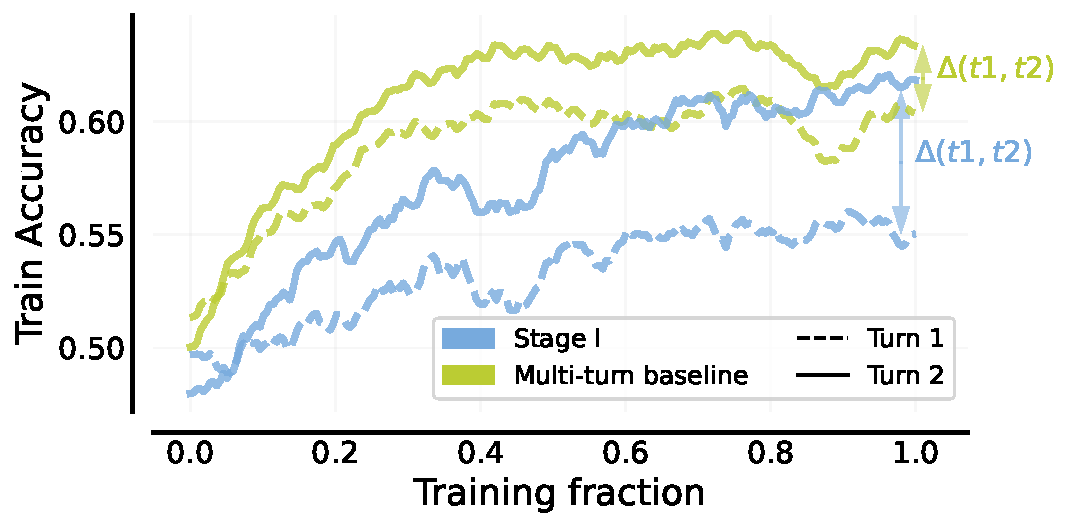
\includegraphics[width=0.99\linewidth]{assets/multiturn_train_stage1_only.pdf}
        \caption{\footnotesize{\textbf{Training accuracy curves.} When training with standard multi-turn RL, the responses at both the attempts become tightly coupled together, leading to poor coverage for subsequent iterations and worse learning progress. Stage I in \methodname{} is explicitly designed to alleviate this and achieves much higher $\Delta$(t1,t2), leading to increased exploration and better final performance.}}
    \end{subfigure}
    ~
    \begin{subfigure}{0.46\linewidth}
        \centering
        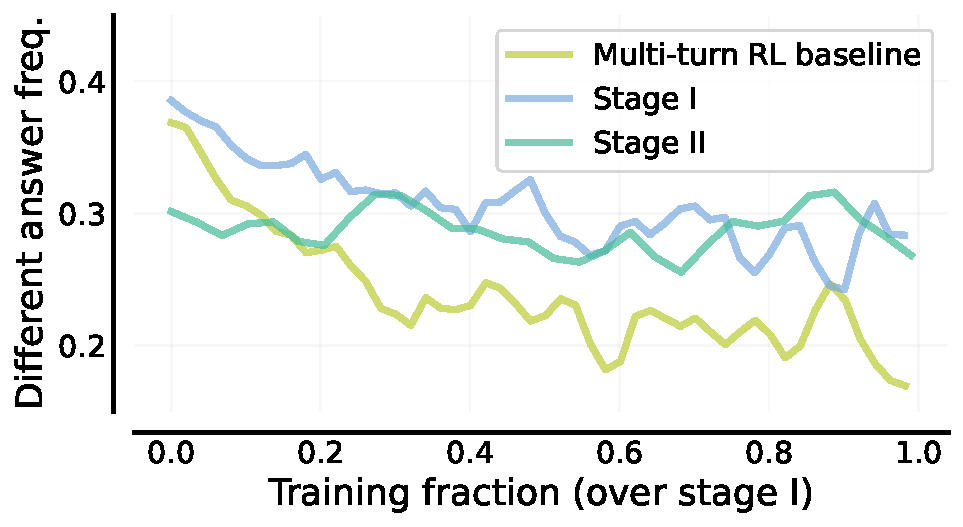
\includegraphics[width=0.99\linewidth]{assets/diff_answer_freq.pdf}
        \caption{\footnotesize{\textbf{Frequency in which the learner proposes a different answer in the second turn.} Without explicitly modifying the policy initialization as in \methodname{}, the policy quickly learns to often not change its answer, leading to poor exploration. Stage I in \methodname{} prevents this issue, and learns non-collapsed behavior in Stage II.}}
        \label{subfig:change_freq}
    \end{subfigure}
    \vspace{-0.2cm}
    \caption{\footnotesize{\textbf{Behavior collapse in standard multi-turn RL} for training self-correction. These results indicate that some explicit approach to avoid collapse is necessary, i.e. Stage I in \methodname{}.}}
    \label{fig:naive_multiturn}
    \vspace{-0.2cm}
\end{figure}

The above results highlight that an effective approach for training LLMs to self-correct entirely via self-generated data must address both distribution shift and behavior collapse. Utilizing on-policy RL is a natural way to address distribution shift, and our method will do so by extending Equation~\ref{eq:base_reinforce} to multiple turns under the hierarchical framework of \citet{zhou2024archer}. However, \textbf{\emph{is behavior collapse an issue for standard multi-turn RL? And if not, how can we address it?}}

To answer these questions, we run standard multi-turn RL training to optimize Equation~\ref{eq:prelims_correctness} only on $(x_2, y_2)$ pairs. Since this objective maximizes the second-attempt performance of the model without training the first attempt, we expect the self-correction $\Delta$(t1,t2) of the model to increase. However, as shown in Figure~\ref{fig:naive_multiturn}, while the performance of each attempt improves with training, their difference $\Delta$(t1, t2) does not. In other words, standard multi-turn RL converges to a state that is overly biased against changing its response, resulting in no self-correction ability and a similar behavior collapse as what we saw with STaR. 

\emph{\textbf{Why does RL still suffer from collapse?}} There are at least two equally good solutions when optimizing a policy with RL on the training data: \textbf{(i)} learning to improve from the first to the second attempt, or \textbf{(ii)} learning to produce the best first-attempt response, followed by no correction in the second attempt. Of course only the former strategy generalizes to new problems, but an overparameterized LLM may not necessarily learn strategy \textbf{(i)} instead of \textbf{(ii)}, since both of these strategies can be equally optimal on \emph{the training set}. Abstractly, learning the ``meta strategy'' of self-correction during training is difficult unless the ``direct'' strategy that optimizes reward appears less viable on the training data. Conceptually, this is similar to the memorization challenge in meta-learning~\citep{yin2019meta}, which suggests that when provided with mutually exclusive tasks, meta-learning is likely to recover the supervised learning solution (without using context from the few shots) that directly predicts the output. Here, this is analogous to not self-correcting past attempts, directly producing an answer.


\begin{figure}[t]
    \centering
    \vspace{-0.1cm}
    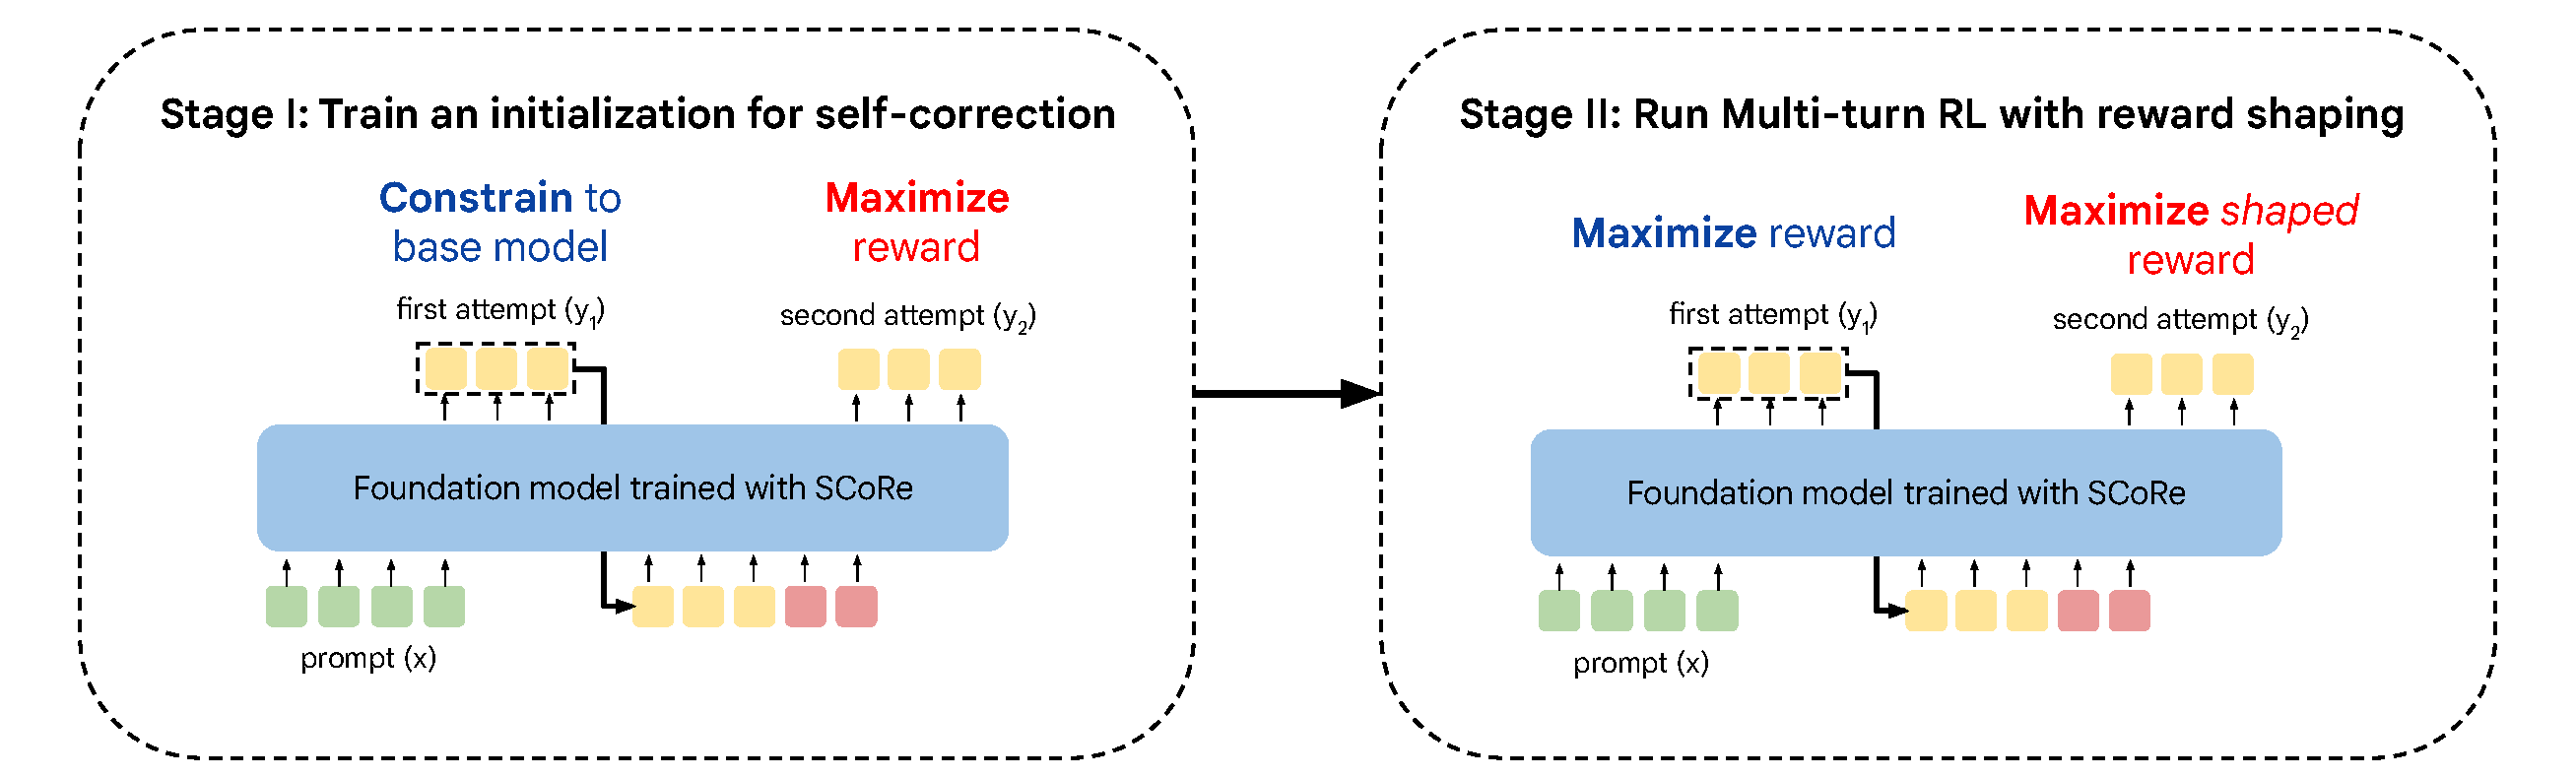
\includegraphics[width=0.95\linewidth]{assets/final_flowchart.pdf}
    \vspace{-0.1cm}
    \caption{\footnotesize{\textbf{An overview of our approach (\methodname{}).} \methodname{} trains a model in two stages: \textbf{Stage I:} instead of running SFT (which produces pathological amplification of biases) to initialize RL training, we train a good initialization that can produce high-reward responses in the second-attempt while mimicking the base model's initial response at the first attempt. \textbf{Stage II:} jointly optimizing both attempts, where the latter uses a shaped reward to incentivize the discovery of the self-correction strategy instead of the simple strategy of producing the best first response followed by making any minor edits to it in the second attempt.}}
    \label{fig:score_flowchart}
    \vspace{-0.3cm}
\end{figure}

\textbf{Method overview.} Although a good self-correcting policy should maximize both accuracy@t1 and accuracy@t2, we saw that standard RL leads to a collapse to non-correcting behavior. Hence, our key insight in \methodname{} is that we must more explicitly encourage self-correction behavior, which we accomplish via a two-stage approach. The first stage (\textbf{Stage I}) serves the role of initialization where we train the model to decouple its behavior across the two attempts by attempting to optimize second-attempt accuracy while explicitly constraining the distribution of first attempts to the base model. From here, \textbf{Stage II} then jointly optimizes the reward of both attempts. To ensure that Stage II does not collapse to the ``direct'' solution, we bias the reward to reinforce self-correction progress. 

\vspace{-0.35cm}
\subsection{Stage I: Training an Initialization that Decouples Attempts}
\vspace{-0.25cm}
The goal of Stage I of \methodname{} is to obtain an initialization by improving the base model's coverage over second attempts given the first attempt, so that subsequent training for self-correction is less prone to behavior collapse. While this would typically be done via SFT, our results in Section~\ref{sec:sft} show that SFT itself suffers from collapse. Therefore, we use RL in this stage to decouple the two attempts.
To do so, we explicitly fine-tune the base model to produce \emph{high-reward} responses at the second attempt, while forcing the model to not change its first attempt by constraining it to be close to the base model using a KL-divergence. While this may appear sub-optimal -- a first attempt with fewer mistakes should lead to a better second attempt -- but as we will show, this stage is critical in reducing the base model's bias towards simply coupling the first and second-attempt distributions, thus avoiding behavior collapse when actual multi-turn RL is run. Formally, the objective is:
\begin{align}
    \label{eq:stage1_loss}
    \max_{\theta}~~ \expected_{\bx_1, \by_1 \sim \pi_{\theta}(\cdot | \bx), \by_2 \sim \pi_\theta(\cdot|[\bx_1, p_1]) }\Big[\widehat{r}(\by_2, \by^*) &- \textcolor{blue}{\beta_2 D_{KL}\left(\pi_{\theta}(\cdot || \bx_1) || \pi_\mathrm{ref}(\cdot | \bx_1)\right)} \Big],
\end{align}
where $\beta_2$ is a hyperparameter designed to enforce a strict KL penalty \emph{\textbf{only on the first attempt}} to avoid shifting of the first-turn responses (denoted by the term in blue). Note that we still utilize the default KL-divergence penalty from Equation~\ref{eq:base_reinforce}, but with a relatively small weight and is omitted from Equation~\ref{eq:stage1_loss} for clarity. Indeed, we show that compared to standard multi-turn RL, Stage I is more effective at decoupling the two responses (Figure~\ref{subfig:change_freq}) and leads to better Stage II performance.

\vspace{-0.2cm}
\subsection{Stage II: Multi-Turn RL with Reward Shaping}
\vspace{-0.2cm}
The second stage of \methodname{} is initialized from Stage I and now jointly optimizes the performance of both attempts. Concretely, Stage II trains the policy $\pi_\theta(\cdot|\cdot)$ using the following objective:
\begin{align}
    \label{eq:two_turn_training}
    \max_{\theta}~~ \expected_{\bx_1, \by_1 \sim \pi_{\theta}(\cdot | \bx), \by_2 \sim \pi_\theta(\cdot|[\bx_1, p_1]) }\left[\sum_{i=1}^2 \widehat{r}(\by_i, \by^*) - \beta_1 D_{KL}\left(\pi_{\theta}(\cdot | \bx_i) || \pi_\mathrm{ref}(\cdot | \bx_i)\right) \right],
\end{align}
where $\bx_i, i \in \{1, 2\}$ corresponds to the set of input tokens passed as context to the model. %

\textbf{Reward shaping to prevent behavior collapse.} In principle, optimizing Equation~\ref{eq:two_turn_training} can also produce a solution that couples responses. This is because we still aim to maximize ground-truth rewards at both attempts. To prevent the learning process from collapsing to a non self-correcting solution in Stage II, we need to bias the learning problem towards self-correction. We implement this via \emph{reward shaping}: by rewarding transitions that make ``progress'' towards learning the desired self-correction behavior. Concretely, given an two-turn rollout sampled from the policy $\tau = \{\bx_1, \hat{\by}_1, \widehat{r}(\by_1, \by^*), \bx_2, \hat{\by}_2, \widehat{r}(\by_2, \by^*) \}$, we modify the reward $\widehat{r}(\by_2, \by^*)$ in Equation~\ref{eq:two_turn_training}, at the second attempt with a bonus $\widehat{b}(\by_2 | \by_1, \by^*) := \alpha \cdot \left(\widehat{r}(\by_2, \by^*) - \widehat{r}(\by_1, \by^*) \right)$,
where $\alpha$ is a positive constant multiplier, ideally larger than 1.0. Adding this bonus to the second attempt measures a notion of progress by \emph{only} emphasizing transitions that flip the correctness of the response and assigns a heavy negative penalty to transitions that change a correct response to incorrect in the second attempt. Thus, the addition of this bonus should regularize the training process from collapsing on to the ``direct'' solution that also appears optimal on the training set but does not learn self-correction.


\vspace{-0.2cm}
\subsection{Putting it Together and Implementation Details} 
\label{sec:hparams}
\vspace{-0.2cm}

Our approach is illustrated pictorially in Figure~\ref{fig:score_flowchart}. We detail all hyperparameters used in Appendix~\ref{app:hparams}. In practice, one can also use an adaptive $\beta_2$ that attempts to balance the magnitudes of the first-attempt KL regularization and the second-attempt policy objective. In some of our experiments, we also choose to amplify the coverage of states used for on-policy RL by incorporating first-attempt solutions obtained by repeatedly sampling the base model as \emph{offline} prompts in RL. We find that incorporating this data, especially in Stage II -- where the first-turn policy may have drifted further from that of the base model -- can have substantial benefits especially when attempting to learn from limited data.

\begin{AIbox}{Takeaways and Implications}
The core insight behind \methodname{} is that we must make it more attractive to learn a more nuanced algorithmic strategy (i.e., self-correction) instead of collapsing to a degenerate behavior mode. To avoid distribution shift, this must be done on self-generated online data. 
\end{AIbox}



